%%%%%%%%%%%%%%%%%%%%%
% A

\appendix
\renewcommand{\thesection}{\arabic{section}}

\chapter{Gannt Diagram}

\begin{figure}[H]
  \centering
    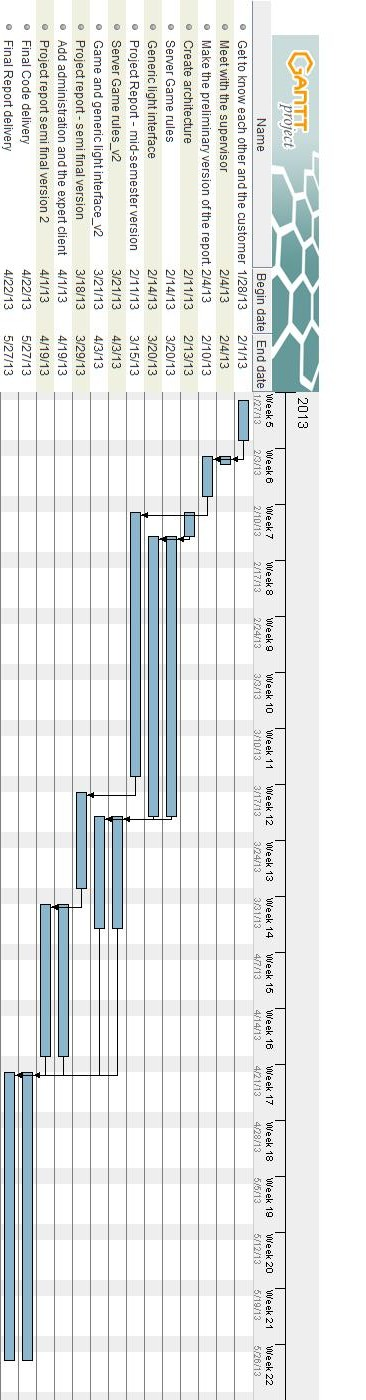
\includegraphics[height=20cm]{img/ganttv3v2.jpg}
  \caption{ 'Gannt diagram'} 
  \label{fig:paperPrototype}
\end{figure}





%%%%%%%%%%%%%%%%%%%%%
% B

\chapter{Don't Panic game rules}
%
\emph{These are the rules of the physical board game, supplied by the customer.}
%
%
\section*{Description of the game}
Don’t Panic is a cooperative game. You start the game as member of a “panic control team”. During your day different potential panicking events will take place and you and your team will have to work together to calm people down and prevent the day from becoming the worst panic event humanity has ever seen. You and your teammates will assume a unique role within the team, with special abilities that will improve your team’s chances, if applied wisely.\\
\\
The aim of the game is to calm the situation down. In the game you can calm people by
\begin{itemize}
	\item opening/blocking paths to help people to get off from frightening situations
	\item talking with them while other solutions are applied
	\item sharing information about how to manage the crisis
	\item moving people from one sector to another. But be careful! You only have a limited time to contain panic.
\end{itemize}
Every 5 minute the “panic level” will increase as a new “panic wave” arrives! If you and your team are unable to keep the panic contained and apply the necessary strategies to calm the people down in time, your city will become a mess and you and your team will lose the game.\\
%
%
\subsection*{A game turn}
The play proceeds clockwise around the table with each player taking turns (in order) until the game ends. For each turn, the current player MUST
\begin{itemize}
	\item take 	4 ACTIONS
	\item draw 	2 INFORMATION CARDS to add to his hand	
	\item draw 	2 EVENT CARDS and perform the corresponding actions on the board
\end{itemize}
%
%
\subsection*{Actions}
A player gets 4 actions to spend on her turn. A given action may be performed more than once during a turn, so long as 1 action is spent for each instance. Each player’s role will grant them special abilities that are unique to that player. Players may also pass if they have nothing else to do. Unused actions CANNOT be saved from turn to turn.\\
\\
In each action the player can
\begin{itemize}
	\item calm 5 people in a sector down
	\item move 5 people from one sector to another
	\item move through a maximum of 3 nodes
	\item create a barrier (is done with the help of another player)	
	\item remove a barrier (is done with the help of another player) 	
	\item decide to spend all his actions in order to create an information center
\end{itemize}
%
%
\subsection*{Components}
1 BOARD represents a real or virtual city. The board is divided into sectors and presents paths and key points. If all the paths in a sector are secured (i.e. blocked) the sector is secured (that is the panic will not augment in the sector at the next wave). However, only a non-secured path can let people pass from one sector to another.\\
\\
8 PAWNS represent the players. The color of the pawn is linked to the draw role card. The pawn moves towards the sectors following key points. The player can act only on the sectors communicating with the key point.\\
\\
1 TIMER calculates the next panic wave. When the timer rings each already panicked sector will be incremented by 5 panicked people (PL). In the non-panicked sectors nothing will happen. During the game panic waves happen initially every 10 minutes, then every 7 minutes and then every 5 minutes.\\
\\
94 PLAYER CARDS :
\begin{itemize}
	\item 6 ROLE CARDS. Each player assumes a specific role in the game which can do particular actions at low cost. The roles are detailed below.
	\item 48 EVENT CARDS. Event cards are, together with the Timer, the source of panic. Each round the player has to draw 2 event cards and apply their effects.
	\item 40 INFORMATION CARDS. Information cards diffuse information which is useful to manage panic. Playing an information card is at 0 cost (i.e. it is an additional action the player can take). Only one card per round can be played and only by the current player. 
\end{itemize}
%
INFORMATION CARDS can be exchanged, but only if the two players are on the same key point. Each round the player has to draw 2 information cards but he can use them only from the next round. Take care! The number of information cards is limited! Once used, they cannot be put back into play.\\
\\
5 INFORMATION CENTERS help lowering the panic. Once an information center has been constructed, the effects of the (draw)?? event cards on the adjacent zone are cut by half. However, creating an information center is a highly costly action. To construct an information center a player needs to use all his actions for this round. A maximum of 5 information centers can be created on a board.\\
\\
DISPLAYS WITH PANIC NUMBERS. Each sector of the game is equipped with a display to indicate the panic level (PL) in the sector. Chain Reactions: Once the panic number reaches quota 50 (that is 50 people panicked in the zone) the panic propagates to all nearby sectors (+5 panicked people). \\
\\
10 BARRIERS help to block the spreading of panic throughout the sectors. To make a zone safe, all the paths have to be blocked. However, people cannot pass through blocked sectors. To create a barrier TWO players have to be on the same key point at the same time. \\
%
%
\subsection*{Sharing Information}
Don’t Panic is a collaborative game! Players are encouraged to openly discuss strategies during the game and share information. An information card can be used only once in a turn but it does not cost any action. Information can be “transferred” from one player to another. To transfer an information card from one player to another, the players have to be on the same key point. Only one card can be transferred at a time. The player who has the role of the Coordinator can transfer a card even if he is not on the same key point. \\
\\
\subsection*{Roles}
Each player is assigned a certain role, and there are six different roles:\\
COORDINATOR : Can share information even if he is not on the same key point\\
CROWD MANAGER: Can calm down 10 people in each sector instead of 5\\
DRIVER: Can move 10 people from one sector to another\\
OPERATION EXPERT: Can create/remove a barrier alone\\
VOLUNTEER: Can support one of the players (apart from the coordinator) duplicating their last action\\
PASSER BY: Can pass 1 information card to a player in an adjacent sector\\
\\
\subsection*{Setting up the game}
\begin{enumerate}
	\item Place the board in the center of the table within easy reach of all the players. Put the displays on the board.
	\item Shuffle the Role cards and deal 1 to each player. Each player takes their corresponding colored pawn. Place the pawn on the big matching colored key point. If the main key point is already taken, choose the small matching colored key point. Put excess Role cards and pawns (if any) back into the box.
	\item Shuffle the INFORMATION CARD cards and deal them to the players face down. For a \\4 PLAYER GAME: 2 CARDS EACH.  \\3 PLAYER GAME: 3 CARDS EACH. \\2 PLAYER GAME: 4 CARDS EACH. \\Place the remaining INFORMATION CARDS face down on the board in the appropriate sector. 	
	\item Shuffle the EVENT CARDS and place them face down on the board in the 	appropriate sector.
	\item Put the initial panic on the board: Each player draws 1 card from the EVENT CARDS and performs the corresponding action.
	\item Turn the INFORMATION CARDS and communicate the possible actions you can perform.
	\item Start the timer.
	\item Play the game! 	
\end{enumerate}

N.B. For a more challenging game session, switch the points 6 and 7. \\
%
\subsection*{Defeat and victory!}
The game ends immediately in defeat for all players if all the map has a panic level higher than 50 panicked people. Players collectively win the game when the panic can no more spread because of the barriers, or if there is no panic on the board.

\section*{User manual}
This is a high level description of how to use the program. When the program starts, the user will have three different choises:

1:	Button - Play

	1.1: A list of active game templates is displayed. Chose one of them, then the program will start a new game with the given template.
	
	1.2: The user can now play the game by moving the players or using actions. 

2: 	Button - Watch replay

	2.1: A list of games that already has been played, is displayed. Chose one of them, then the program will enter the given replay.
	
	2.2: Press the "next" button to show the next action.

3:	Button - Expert interface

	The expert interface is used to set up the game before it is played. 
		
	Button - Add effect, set wanted effect.
	
	Button - Add role, set wanted role.
	
	Button - Add player, set role and startnode for the player.

	Button - Start!, starts the canvas so the user can create the map.

	Mouse click on canvas - adds a new node to the map. 

	Button - Delete node, deletes the selected node from the map.
	
	Button - Start node connection, starts a node connection in the selected zone and connects it to the next node that is selected.
	
	Button - Add zone node, adds a node to a zone. 
	
	Button - Clear zone node, removes a node from a zone. 
	
	Button - Create zone, creates a zone if the nodes around it are zone nodes.
	
	Button - Delete zone, deletes the selected zone.
	
	Button - Set people, sets how many people in the selected zone.
	
 	Button - Set panic, sets the panic level in the selected zone. 

%%%%%%%%%%%%%%%%%%%%%%
% C

\chapter{Description of the Sifteo Cubes}

\textbf{Taken from the Sifteo FAQ}


\section{How do Sifteo Cubes work?}
Sifteo Cubes is a hands-on interactive game system. They communicate wirelessly to respond to each other and being tilted, shaken, flipped, and pressed. The Sifteo Base stores your games and plays audio. You can play with 3-12 Sifteo cubes at once!\\
Sifteo Cubes use 1 AAA battery each. Sifteo Bases use 2 AAA batteries. Rechargeable nickel metal hydride (NiMH) batteries, standard alkaline, or lithium (non-rechargeable) batteries will each work. Batteries last for approximately 8 hours of gameplay.

\section{Who are Sifteo Cubes for?}
Sifteo Cubes are perfect for kids and kids at heart who geek out on brainy challenging games and cool new gadgets (recommended for ages 7 to adult). Our games can be played individually and with friends and family. Sifteo Cubes are sturdy and can withstand some abuse. Still, they are sophisticated electronic devices, and very rough handling (throwing, dunking in water, and other forms of cube torture) can break a cube permanently.

\section{How do I play games on my cubes?}
Sifteo Cubes come pre-installed with 4 games that work right out of the box. You can buy more games using the Sifteo desktop software (download here) and install them by connecting the Sifteo Base to your computer with the USB cable that comes with it. Sifteo games are 80-120 credits (about $8-$12) each. You can buy credits through the desktop software.
View full tech specs and system requirements here .

